% =============================================================================
% HQC-on-RISC-V — Παρουσίαση Διπλωματικής (15' defense deck)
% Engine: LuaLaTeX · Theme: metropolis 16:9 · Build: `make` (see README.md)
% =============================================================================
\documentclass[aspectratio=169,10pt]{beamer}

% =============================================================================
% preamble.tex — shared preamble for the HQC-on-RISC-V defense deck
% Engine: LuaLaTeX (see .latexmkrc / Makefile). Theme: metropolis, 16:9, 10pt.
% -----------------------------------------------------------------------------
% CLASS-COUPLING GUARD: this deck is `beamer`, NOT the thesis `scrbook`.
% We deliberately DO NOT \input the thesis preamble (packages/settings/macros).
% We replicate ONLY the macros the reused figures + slides need, and \input the
% thesis figure DESIGN SYSTEM (../figures/thesis-tikz-styles.tex) which is
% class-agnostic (colour + \tikzset + \pgfplotsset + tabularray specs only).
%
% NOTE: this deck does NOT load biblatex (it cites nothing). If you previously
% built a biblatex-enabled version, delete build/ first (`make distclean`):
% a stale build/main.aux with \abx@aux@refcontext is a fatal undefined-cs error.
% =============================================================================

\usetheme[progressbar=frametitle,numbering=fraction,sectionpage=progressbar]{metropolis}

% --- Fonts & language (match thesis: Libertinus + Greek/English) -------------
\usepackage{fontspec}
\usepackage{unicode-math}
\setmainfont{Libertinus Serif}
\setsansfont{Libertinus Sans}
\setmonofont{Fira Mono}[Scale=MatchLowercase]
\setmathfont{Libertinus Math}
\usepackage{polyglossia}
\setdefaultlanguage[variant=monotonic]{greek}
\setotherlanguage{english}
% Greek monospace fallback (Fira Mono lacks Greek glyphs)
\newfontfamily\greekfonttt{DejaVu Sans Mono}[Scale=MatchLowercase]
\newcommand{\en}[1]{\textenglish{#1}}

% --- siunitx + tables/graphics required by the reused thesis figures ---------
\usepackage{xspace}
\usepackage{booktabs}
\usepackage{siunitx}
\sisetup{detect-all, group-separator={\,}, group-minimum-digits=4}
\usepackage{tabularray}
\UseTblrLibrary{booktabs}
\usepackage{graphicx}
\usepackage{pgfplots}
\pgfplotsset{compat=1.18}
\usetikzlibrary{arrows.meta, calc, decorations.pathreplacing, external,
  fit, matrix, positioning, shapes.geometric, shapes.misc}
% NOTE: `external` is loaded only so reused figures' \tikzsetnextfilename{...}
% is defined. We do NOT call \tikzexternalize, so it is a harmless no-op here.

% --- Accent colour shared with the reused figures (must precede the \input) --
\definecolor{thesisblue}{RGB}{10,40,80}

% --- Semantic slide colours (skill spec) -------------------------------------
\definecolor{posgreen}{HTML}{1B7837}
\definecolor{conred}{HTML}{B2182B}
\definecolor{hlblue}{HTML}{2166AC}
\newcommand{\pos}[1]{\textcolor{posgreen}{#1}}
\newcommand{\con}[1]{\textcolor{conred}{#1}}
\newcommand{\HL}[1]{\textcolor{hlblue}{#1}}

% --- metropolis accents -> thesis navy ---------------------------------------
\setbeamercolor{frametitle}{bg=thesisblue}
\setbeamercolor{progress bar}{fg=hlblue}
\setbeamercolor{title separator}{fg=hlblue}

% --- Thesis figure DESIGN SYSTEM (colour + tikz styles; class-agnostic) ------
% Single source of truth: lets reused \input figures resolve figT/*, figedge,
% fignode/*, figkPolymul, oi* colours, figlegend, etc. Requires \thesisblue +
% pgfplots + tabularray + the tikz libs above (all loaded). The file is
% documented as redefinition-safe and only defines colours/styles.
\input{../figures/thesis-tikz-styles}

% --- Macro subset replicated from thesis preamble/macros.tex -----------------
% (Deck is beamer, not scrbook: never \input the thesis preamble wholesale.)
\newcommand{\HQC}{\textsc{HQC}\xspace}
\newcommand{\KeyGen}{\textsc{KeyGen}\xspace}
\newcommand{\Encaps}{\textsc{Encaps}\xspace}
\newcommand{\Decaps}{\textsc{Decaps}\xspace}
\newcommand{\ext}[1]{\textsf{#1}}
\newcommand{\insn}[1]{\texttt{#1}\xspace}
\newcommand{\clmul}{\insn{clmul}}
\newcommand{\clmulh}{\insn{clmulh}}
\newcommand{\vclmul}{\insn{vclmul.vx}}
\newcommand{\vclmulh}{\insn{vclmulh.vx}}
\newcommand{\vror}{\insn{vror}}
\newcommand{\rori}{\insn{rori}}
\newcommand{\Zbc}{\ext{Zbc}\xspace}
\newcommand{\Zbb}{\ext{Zbb}\xspace}
\newcommand{\Zba}{\ext{Zba}\xspace}
\newcommand{\Zvbc}{\ext{Zvbc}\xspace}
\newcommand{\Zvbb}{\ext{Zvbb}\xspace}
\newcommand{\RVV}{\textsc{RVV}\xspace}
\newcommand{\instret}{\texttt{instret}\xspace}
\newcommand{\VLEN}{\texttt{VLEN}\xspace}
\newcommand{\code}[1]{\texttt{#1}}
\newcommand{\speedup}[1]{$\times$#1}
\newcommand{\insnreduction}[1]{$\times$#1}
\newcommand{\cycles}[1]{\num{#1}}
\newcommand{\pct}[1]{\SI{#1}{\percent}}

% --- Title metadata ----------------------------------------------------------
% (Title/subtitle use only zero-arg macros; plain-text author avoids the
%  hyperref "token not allowed in PDF string" warning from a thin space.)
\title{Επιτάχυνση του Μετα-Κβαντικού KEM \HQC σε Αρχιτεκτονική RISC-V}
\subtitle{Επιτάχυνση μέσω Επεκτάσεων ISA — \Zbc/\Zbb, \Zvbc/\Zvbb}
\author{Φραϊδάκης Ιωάννης (ΑΕΜ 10736)}
\institute{%
  Αριστοτέλειο Πανεπιστήμιο Θεσσαλονίκης\\
  Τμήμα Ηλεκτρολόγων Μηχανικών \& Μηχανικών Υπολογιστών\\[0.5em]
  {\footnotesize Επιβλέπων: Καθ. Ιωάννης Παπαευσταθίου\\
   Τριμελής επιτροπή: Β. Παυλίδης, Α. Χατζόπουλος}%
}
\date{Θεσσαλονίκη, Ιούνιος 2026}


\begin{document}

% --- Title slide -------------------------------------------------------------
\begin{frame}[plain]
  \maketitle
\end{frame}

% --- Outline -----------------------------------------------------------------
\begin{frame}{Διάρθρωση}
  \tableofcontents[hideallsubsections]
\end{frame}

\section{Κίνητρο \& Υπόβαθρο}
\begin{frame}{Το κίνητρο: η κβαντική απειλή}
  \begin{columns}[T]
    \begin{column}{0.46\textwidth}
      \begin{itemize}
        \item Ο \en{Shor} σπάει \en{RSA}/\en{ECC} σε πολυωνυμικό χρόνο.
        \item \con{Harvest-now, decrypt-later}: τα δεδομένα κινδυνεύουν \emph{σήμερα}.
        \item \en{NIST PQC} $\rightarrow$ \en{CNSA 2.0}: μετάβαση έως το \HL{2035}.
        \item Το \HQC επιλέχθηκε από το \en{NIST} (2025) ως \en{code-based KEM}.
      \end{itemize}
    \end{column}
    \begin{column}{0.54\textwidth}
      \resizebox{\linewidth}{!}{\input{../figures/ch1-introduction/timeline-pqc}}
    \end{column}
  \end{columns}
\end{frame}

\begin{frame}{\HQC: ένα \en{code-based KEM}}
  \begin{columns}[T]
    \begin{column}{0.40\textwidth}
      \begin{itemize}
        \item Τρεις πράξεις: \KeyGen, \Encaps, \Decaps.
        \item Πυρήνας: πολυωνυμικός πολλαπλασιασμός στο $\mathbb{F}_2[x]/(x^n-1)$.
        \item \en{Keccak/SHAKE} για δειγματοληψία \& \en{FO} μετασχηματισμό.
        \item Αποκωδικοποίηση συνένωσης \en{RM}+\en{RS}.
      \end{itemize}
    \end{column}
    \begin{column}{0.60\textwidth}
      \resizebox{\linewidth}{!}{\input{../figures/ch2-background/hqc-dataflow}}
    \end{column}
  \end{columns}
\end{frame}

\begin{frame}{Πλατφόρμα: επεκτάσεις ISA της RISC-V}
  \begin{columns}[T]
    \begin{column}{0.42\textwidth}
      \begin{itemize}
        \item \textbf{Scalar:} \Zbc/\Zbb — \clmul carry-less πολλαπλασιασμός.
        \item \textbf{Vector (\RVV):} ευρεία δεδομένα, \en{vector-length agnostic}.
        \item \textbf{Vector-crypto:} \Zvbc/\Zvbb — \vclmul.
        \item Τρία \en{deployment tiers} = σταδιακή υιοθέτηση ISA.
      \end{itemize}
    \end{column}
    \begin{column}{0.58\textwidth}
      \resizebox{\linewidth}{!}{\input{../figures/ch6-polymul/polymul-tiers}}
    \end{column}
  \end{columns}
\end{frame}


\section{Πρόβλημα \& Προσέγγιση}
\begin{frame}{Πού ξοδεύεται ο χρόνος;}
  \begin{columns}[T]
    \begin{column}{0.42\textwidth}
      \begin{itemize}
        \item Ο πολυωνυμικός πολλαπλασιασμός είναι \HL{${\sim}97\%$} του \instret.
        \item scalar reference, HQC-128.
        \item Άρα: η βελτιστοποίηση ξεκινά από εκεί.
        \item Δευτερεύοντες πυρήνες: \en{Keccak}, αποκωδικοποίηση.
      \end{itemize}
    \end{column}
    \begin{column}{0.58\textwidth}
      \resizebox{\linewidth}{!}{\input{../figures/ch2-background/pie-scalar-ref}}
    \end{column}
  \end{columns}
\end{frame}

\begin{frame}{Προσέγγιση: από bit-serial σε word-level}
  \begin{itemize}
    \item \en{Karatsuba} \en{compile-time specialized fixed-tree} code generation για $\mathbb{F}_2[x]$.
    \item Φύλλα δέντρου: αντικατάσταση $64\times n^2$ shift-XOR με \clmul/\clmulh.
  \end{itemize}
  \vspace{0.2em}
  \begin{center}
    \resizebox{0.9\linewidth}{!}{\input{../figures/ch6-polymul/schoolbook-vs-clmul}}
  \end{center}
\end{frame}

\begin{frame}{Tier 1 — Scalar (\Zbc/\Zbb)}
  % src: results/reports/summaries/speedups_simulation.md (Table 1)
  \begin{itemize}
    \item \en{polymul}: \num{18639752} $\rightarrow$ \num{186629} \instret (HQC-128).
    \item \pos{\speedup{99.9}} στο \en{polymul}· \pos{\speedup{34}} στο πλήρες HQC-128 \en{KEM}.
    \item Καθαρό λογισμικό — καμία custom hardware μονάδα.
    \item \en{Deployment}: \en{IoT}-class \en{rv64gc} + bit-manip επεκτάσεις.
  \end{itemize}
\end{frame}

\begin{frame}{Tier 2/3 — Διανυσματική επιτάχυνση}
  % src: results/reports/summaries/speedups_simulation.md (Tables 2-3, polymul)
  \begin{columns}[T]
    \begin{column}{0.46\textwidth}
      \begin{itemize}
        \item \textbf{Tier 2 (\RVV):} vectorized \en{Karatsuba} φύλλα $\rightarrow$ \pos{\speedup{125}} \en{polymul}.
        \item \textbf{Tier 3 (\Zvbc):} \vclmul $\rightarrow$ \pos{\speedup{264}} \en{polymul} (HQC-128).
        \item Υβριδική αρχιτεκτονική: \RVV \en{polymul} + scalar \en{Keccak} (αποφυγή \en{rotation penalty}).
      \end{itemize}
    \end{column}
    \begin{column}{0.54\textwidth}
      \resizebox{\linewidth}{!}{\input{../figures/ch6-polymul/vclmul-leaf-dataflow}}
    \end{column}
  \end{columns}
\end{frame}

\begin{frame}{Βοηθητικοί πυρήνες: \en{Keccak} \& αποκωδικοποίηση}
  % src: results/reports/summaries/speedups_simulation.md (Tables 4-5)
  \begin{columns}[T]
    \begin{column}{0.5\textwidth}
      \textbf{\en{Keccak}/SHA-3}
      \begin{itemize}
        \item 2-way \en{SoA} με \Zvbb (\vror).
        \item \pos{\speedup{1.36}}–\pos{\speedup{1.37}}.
      \end{itemize}
    \end{column}
    \begin{column}{0.5\textwidth}
      \textbf{Αποκωδικοποίηση \en{RM}+\en{RS}}
      \begin{itemize}
        \item \RVV + \Zvbc $\mathrm{GF}(2^8)$.
        \item \pos{\speedup{13.2}}–\pos{\speedup{15.9}}.
      \end{itemize}
    \end{column}
  \end{columns}
  \vspace{0.4em}
  \begin{center}\footnotesize Μετά τον \en{polymul}, οι πυρήνες αυτοί κυριαρχούν στο εναπομείναν κόστος.\end{center}
\end{frame}


\section{Πειράματα \& Αποτελέσματα}
\begin{frame}{Πειραματική διάταξη}
  \begin{itemize}
    \item \textbf{Εξομοίωση:} \en{Spike ISS} — ντετερμινιστικό \instret (όλα τα tiers).
    \item \textbf{Hardware:} \en{Banana Pi BPI-F3} (\en{SpacemiT K1 X60}, \VLEN${}=256$) — κύκλοι ρολογιού.
    \item \en{KAT}-validated ορθότητα· median, single-core pinning.
    \item \con{Tier 3 μόνο σε εξομοίωση} — απουσία silicon με \Zvbc.
  \end{itemize}
  \vfill
  \begin{center}\footnotesize
    \instret = αριθμός δυναμικά εκτελεσθεισών εντολών · κάτω φράγμα κύκλων σε in-order pipelines.
  \end{center}
\end{frame}

\begin{frame}{Αποτελέσματα: επιτάχυνση πλήρους \en{KEM}}
  \begin{columns}[T]
    \begin{column}{0.58\textwidth}
      \tikzsetnextfilename{pres-results-kem-speedups}
      % src: results/reports/summaries/speedups_simulation.md
      %      Total KEM, Speedup = scalar_ref instret / champion instret (HQC-128)
      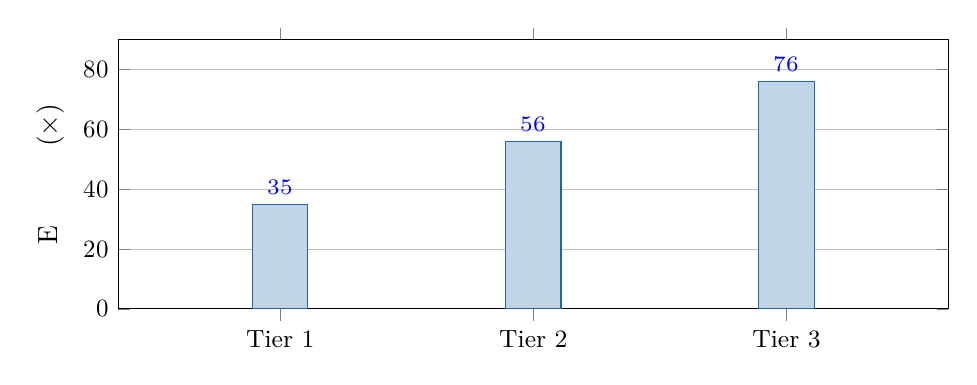
\begin{tikzpicture}
        \begin{axis}[
          width=\linewidth, height=5.0cm,
          ybar, bar width=20pt,
          ymin=0, ymax=90,
          ylabel={Επιτάχυνση ($\times$)},
          symbolic x coords={Tier 1, Tier 2, Tier 3},
          xtick=data,
          nodes near coords,
          every node near coord/.append style={font=\footnotesize,
            /pgf/number format/fixed, /pgf/number format/precision=0},
          enlarge x limits=0.32,
          tick label style={font=\small},
          ymajorgrids=true,
        ]
          \addplot+[draw=hlblue, fill=hlblue!28]
            coordinates {(Tier 1,35.0) (Tier 2,55.9) (Tier 3,75.9)};
        \end{axis}
      \end{tikzpicture}
    \end{column}
    \begin{column}{0.42\textwidth}
      \footnotesize HQC-128, \instret (\en{Spike}).
      \begin{itemize}
        \item Tier 1 (scalar): \pos{\speedup{35}}
        \item Tier 2 (\RVV): \pos{\speedup{56}}
        \item Tier 3 (\Zvbc): \pos{\speedup{76}}
      \end{itemize}
      \pause
      \vspace{0.3em}
      \textbf{Κορυφή HQC-256:} \pos{\speedup{164}} \en{KEM}, \pos{\speedup{436}} \en{polymul}.
    \end{column}
  \end{columns}
\end{frame}

\begin{frame}{Σύγκριση με state-of-the-art}
  \begin{itemize}
    \item Tier 3 \instret (HQC-128 \en{KEM}) $=$ \num{702755}, ίδια τάξη μεγέθους με τον \en{x86-64 FFT+CRT} champion.
    \item Σε εκτιμώμενους κύκλους, χάσμα $\approx 2.7\times$ (ωριμότητα \en{AVX2}).
    \item \con{Προσοχή:} \instret (εξομοίωση) έναντι κύκλων (hardware), όχι άμεσα ισοδύναμα.
    \item \en{Hardware} (BPI-F3, Tier 1): \pos{\speedup{34}} πλήρες \en{KEM}, επιβεβαιώνει την εξομοίωση.
  \end{itemize}
\end{frame}


\section{Συμπεράσματα}
\begin{frame}{Συμπεράσματα}
  \begin{itemize}
    \item Πρώτη πλήρως βελτιστοποιημένη υλοποίηση \HQC σε RISC-V, καθαρό λογισμικό.
    \item Τρία tiers: \pos{\speedup{34}} $\rightarrow$ \pos{\speedup{60}} $\rightarrow$ \pos{\speedup{167}} (HQC-128 \en{KEM}).
    \item \textbf{ISA completeness $>$ ISA width}: η σωστή εντολή (\clmul, \vror) αξίζει περισσότερο από ευρύτερους καταχωρητές.
    \item \en{Constant-time}: αρχιτεκτονική ανάλυση \en{Zkt} + εμπειρικό \en{dudect} (Tier 1/2).
  \end{itemize}
\end{frame}

\begin{frame}{Περιορισμοί \& μελλοντική εργασία}
  \begin{itemize}
    \item \con{Tier 3} χωρίς hardware validation (απουσία \Zvbc silicon).
    \item Εμπειρικό \en{CT} μόνο για Tier 1/2· Tier 3 \en{CT} ανοιχτό.
    \item \instret $\neq$ κύκλοι — άμεση cross-arch σύγκριση με επιφυλάξεις.
    \item Μελλοντικά: silicon \Zvbc, formal \en{CT}, multi-core αξιολόγηση.
  \end{itemize}
  \vspace{0.7em}
  \begin{center}\Large Ευχαριστώ — Ερωτήσεις;\end{center}
\end{frame}


% --- Backup (after \appendix: excluded from the main progress count) ---------
\appendix
% =============================================================================
% Backup slides — μετά το \appendix (εκτός κύριας ροής και progress count)
% Όλα τα νούμερα: results/reports/summaries/speedups_simulation.md & speedups_hardware.md
% =============================================================================

\begin{frame}{Backup — Πλήρης πίνακας επιταχύνσεων \en{KEM} (\instret)}
  \small
  \begin{center}
  \begin{tabular}{lccc}
    \toprule
    & Tier 1 & Tier 2 & Tier 3 \\
    \midrule
    HQC-128 & \speedup{35.0} & \speedup{55.9} & \speedup{75.9} \\
    HQC-192 & \speedup{46.9} & \speedup{72.3} & \speedup{107.0} \\
    HQC-256 & \speedup{60.1} & \speedup{86.9} & \speedup{163.8} \\
    \bottomrule
  \end{tabular}
  \end{center}
  \vspace{0.4em}
  \footnotesize \en{polymul} (HQC-128): \speedup{101.3}/\speedup{124.6}/\speedup{264.1}.
  HQC-256: \speedup{110.2}/\speedup{133.4}/\speedup{436.5}.
\end{frame}

\begin{frame}{Backup — \en{Keccak} \& αποκωδικοποίηση}
  \small
  \begin{center}
  \begin{tabular}{lccc}
    \toprule
    Επιτάχυνση & HQC-128 & HQC-192 & HQC-256 \\
    \midrule
    \en{Keccak} & \speedup{1.37} & \speedup{1.36} & \speedup{1.36} \\
    \en{Decode} & \speedup{14.3} & \speedup{15.9} & \speedup{13.2} \\
    \bottomrule
  \end{tabular}
  \end{center}
\end{frame}

\ifincludeCT
\begin{frame}{Backup — \en{Constant-time} ασφάλεια}
  \begin{itemize}
    \item Αρχιτεκτονική ανάλυση \en{Zkt}: κάθε εντολή στο data-independent timing subset.
    \item Εμπειρικό \en{dudect} σε BPI-F3: \code{scalar\_ref}, \code{scalar\_zb}, \code{vector\_rvv}.
    \item Tier 3 (\code{vector\_zvk}): θεωρητική \en{CT}, εκκρεμεί silicon.
  \end{itemize}
\end{frame}
\fi

\begin{frame}{Backup — \en{Hardware} (BPI-F3, HQC-128)}
  \small
  \begin{center}
  \begin{tabular}{lcc}
    \toprule
    & scalar (\Zbc) & vector (\RVV) \\
    \midrule
    \en{polymul} & \speedup{95.0} & \speedup{95.3} \\
    Πλήρες \en{KEM} & \speedup{37.5} & \speedup{45.9} \\
    \bottomrule
  \end{tabular}
  \end{center}
  \par\vspace{0.3em}
  \footnotesize \en{IPC}$\approx 1.49$, ο \instret υπερεκτιμά τους κύκλους κατά ${\approx}$\pct{50}.
\end{frame}


\end{document}
